
        \documentclass[spanish, 11pt]{exam}

        %These tell TeX which packages to use.
        \usepackage{array,epsfig}
        \usepackage{amsmath, textcomp}
        \usepackage{amsfonts}
        \usepackage{amssymb}
        \usepackage{amsxtra}
        \usepackage{amsthm}
        \usepackage{mathrsfs}
        \usepackage{color}
        \usepackage{multicol, xparse}
        \usepackage{verbatim}


        \usepackage[utf8]{inputenc}
        \usepackage[spanish]{babel}
        \usepackage{eurosym}

        \usepackage{graphicx}
        \graphicspath{{../img/}}



        \printanswers
        \nopointsinmargin
        \pointformat{}

        %Pagination stuff.
        %\setlength{\topmargin}{-.3 in}
        %\setlength{\oddsidemargin}{0in}
        %\setlength{\evensidemargin}{0in}
        %\setlength{\textheight}{9.in}
        %\setlength{\textwidth}{6.5in}
        %\pagestyle{empty}

        \let\multicolmulticols\multicols
        \let\endmulticolmulticols\endmulticols
        \RenewDocumentEnvironment{multicols}{mO{}}
         {%
          \ifnum#1=1
            #2%
          \else % More than 1 column
            \multicolmulticols{#1}[#2]
          \fi
         }
         {%
          \ifnum#1=1
          \else % More than 1 column
            \endmulticolmulticols
          \fi
         }
        \renewcommand{\solutiontitle}{\noindent\textbf{Sol:}\enspace}

        \newcommand{\samedir}{\mathbin{\!/\mkern-5mu/\!}}

        \newcommand{\class}{1º Bachillerato}
        \newcommand{\examdate}{\today}

        \newcommand{\tipo}{A}


        \newcommand{\timelimit}{50 minutos}



        \pagestyle{head}
        \firstpageheader{
\includegraphics[width=0.2\columnwidth]{header_left}}{\textbf{Departamento de Matemáticas\linebreak \class}\linebreak \examnum}{
\includegraphics[width=0.1\columnwidth]{header_right}}
        \runningheader{\class}{\examnum}{Página \thepage\ of \numpages}
        \runningheadrule

        \newcommand{\examnum}{Ejercicios de Estadística Unidimensional}
        \begin{document}
        \begin{questions}
        \question p089e01 - Se realiza una encuesta a un grupo de 20 personas acerca del número de veces que acuden al cine alo largo de un año, obteniéndose los siguientes resultados:0 1 2 3 3 2 0 1 1 1 2 2 1 0 0 0 0 1 2 3
        \begin{multicols}{1} 
        \begin{parts} \part[1] Realiza una tabla de frecuencias  \begin{solution}   \begin{tabular}{rrrrrrr}
\hline
   x\_i &   f\_i &   F\_i &   h\_i &   H\_i &   \%\_i &   \%A\_i \\
\hline
     0 &     6 &     6 &  0.3  &  0.3  &    30 &     30 \\
     1 &     6 &    12 &  0.3  &  0.6  &    30 &     60 \\
     2 &     5 &    17 &  0.25 &  0.85 &    25 &     85 \\
     3 &     3 &    20 &  0.15 &  1    &    15 &    100 \\
\hline
\end{tabular}   \end{solution} \part[1] Realiza un diagrama de barras y un polígono de frecuencias  \begin{solution}   \\ 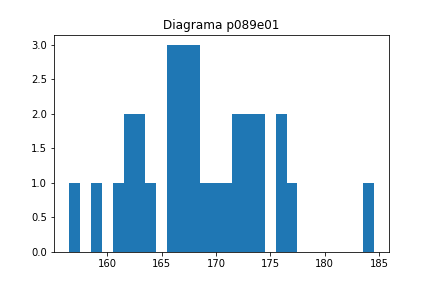
\includegraphics[width=1\columnwidth]{p089e01}   \end{solution} \part[1] Calcular los parámetros de centralización  \begin{solution}   {'media': 1.25, 'mediana': 1.0, 'moda': ModeResult(mode=array([0]), count=array([6]))}   \end{solution} \part[1] Calcular los parámetros de posición P70, Q1, Q3, D4  \begin{solution}   {'P70': 2.0, 'Q1': 0.0, 'Q3': 2.0, 'D4': 1.0}   \end{solution} \part[1] Calcular los parámetros de dispersión  \begin{solution}   {'rango': 3, 'varianza': 1.0875, 'desviación típica': 1.04283268073071, 'coeficiente variación': 0.834266144584568}   \end{solution}
        \end{parts}
        \end{multicols}
        
    \end{questions}
    \end{document}
    